% !TEX encoding = UTF-8
% !TEX TS-program = pdflatex
% !TEX root = ../Tesi.tex
% !TEX spellcheck = en-EN

%************************************************
\chapter{Sinter Segregator}
\label{cap:sintersegregator}
%************************************************

\info{available sketches and images from the Primetals presentation.}
There are two main phases:
\begin{itemize}
  \item{Initial filling: during this phase many small particles deposited inside
  the chute}
  \item{Moving bottom box: also in this phase particles were
continuously inserted from the top. After the filling was completed, the
scraper was moved and all the particles further a defined surface were
deleted. Inside the sinter, all the places that small particles could
occupy already were. At this point the bottom box was filled again, but
with a more realistic size distribution, and it reached steady state, as can
be seen in figures \ref{fig:043rS1}, \ref{fig:044rS2}, \ref{fig:045rS4}, and
\ref{fig:046rS6}.}
\end{itemize}
As expected, when the steady state was reached, the particles actually
segregated, as it was intended to demonstrate.
In fact, there were more particles with larger radiuses, from 8 to 25 mm, in the
bottom layers.
Instead, the smallest particles, radius = 2.5 mm, was rather on the top layer. 
\begin{figure}%[!htb] 
\centering 
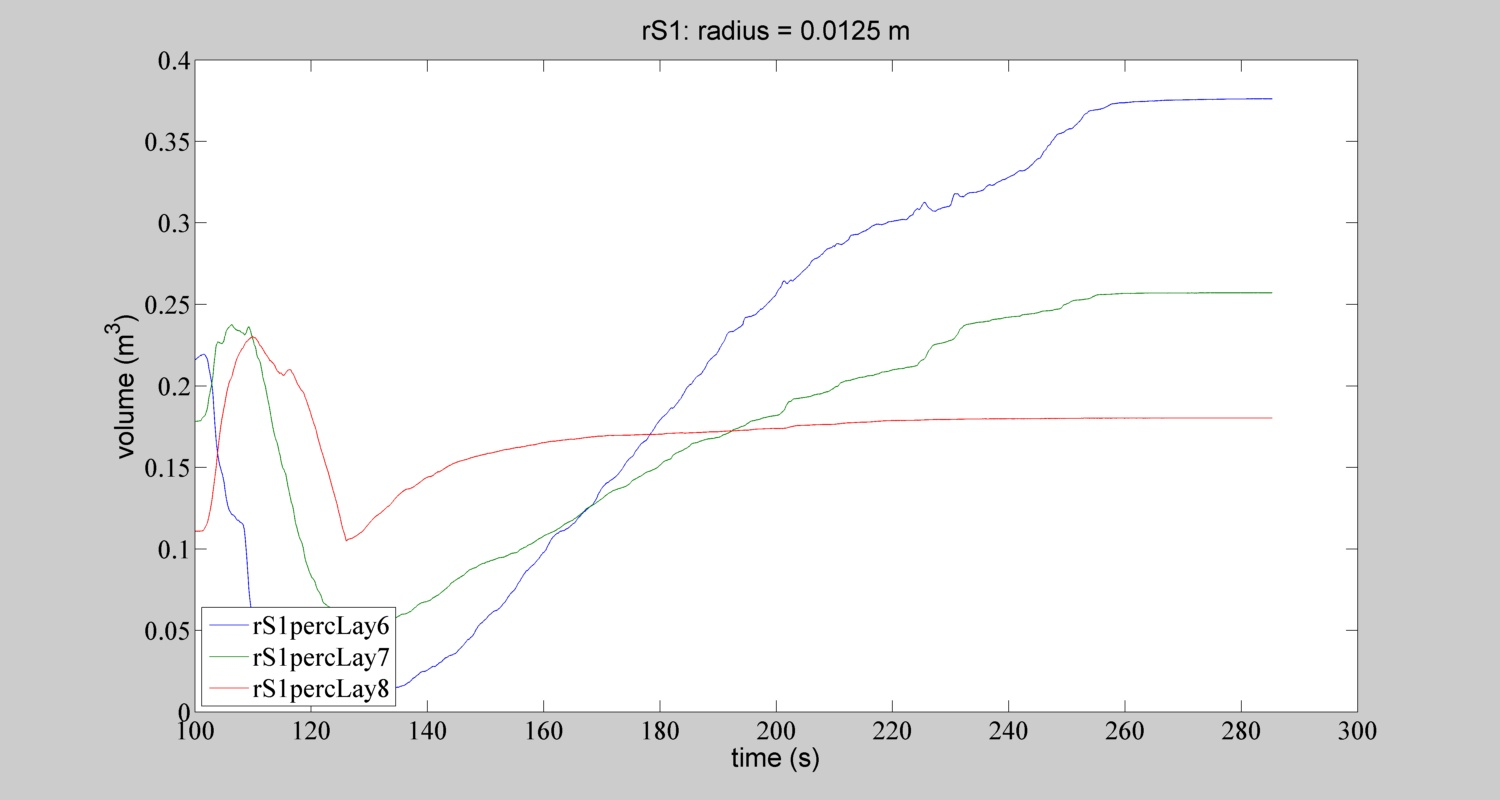
\includegraphics[width=.48\columnwidth]{images/043rS1} 
\caption{Radius 1}
\label{fig:043rS1} 
\end{figure}
%************************************************
\begin{figure}%[!htb] 
\centering 
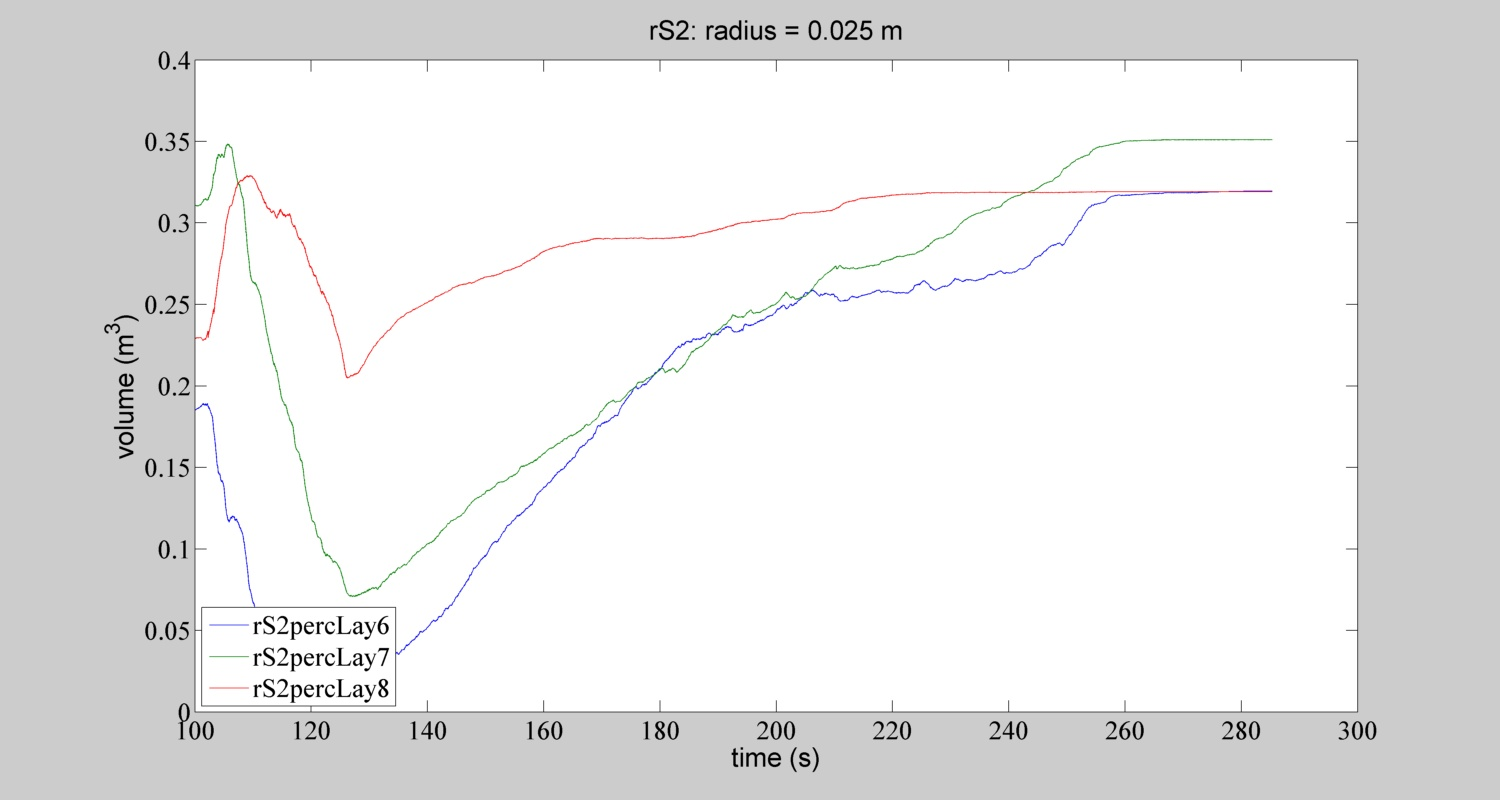
\includegraphics[width=.48\columnwidth]{images/044rS2} 
\caption{Radius 2}
\label{fig:044rS2} 
\end{figure}
%************************************************
\begin{figure}%[!htb] 
\centering 
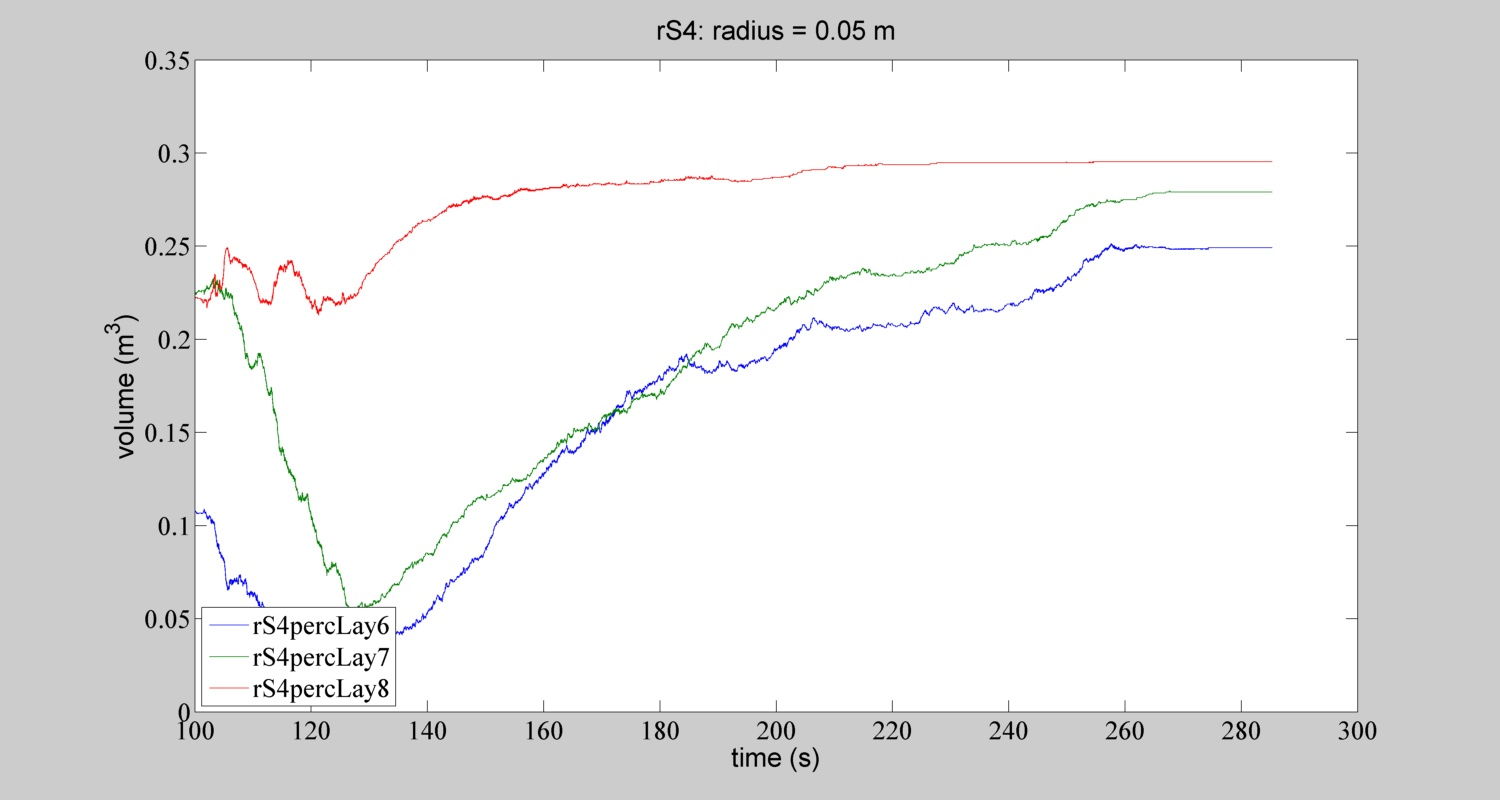
\includegraphics[width=.48\columnwidth]{images/045rS4}
\caption{Radius 4}
\label{fig:045rS4} 
\end{figure}
%************************************************
\begin{figure}%[!htb] 
\centering 
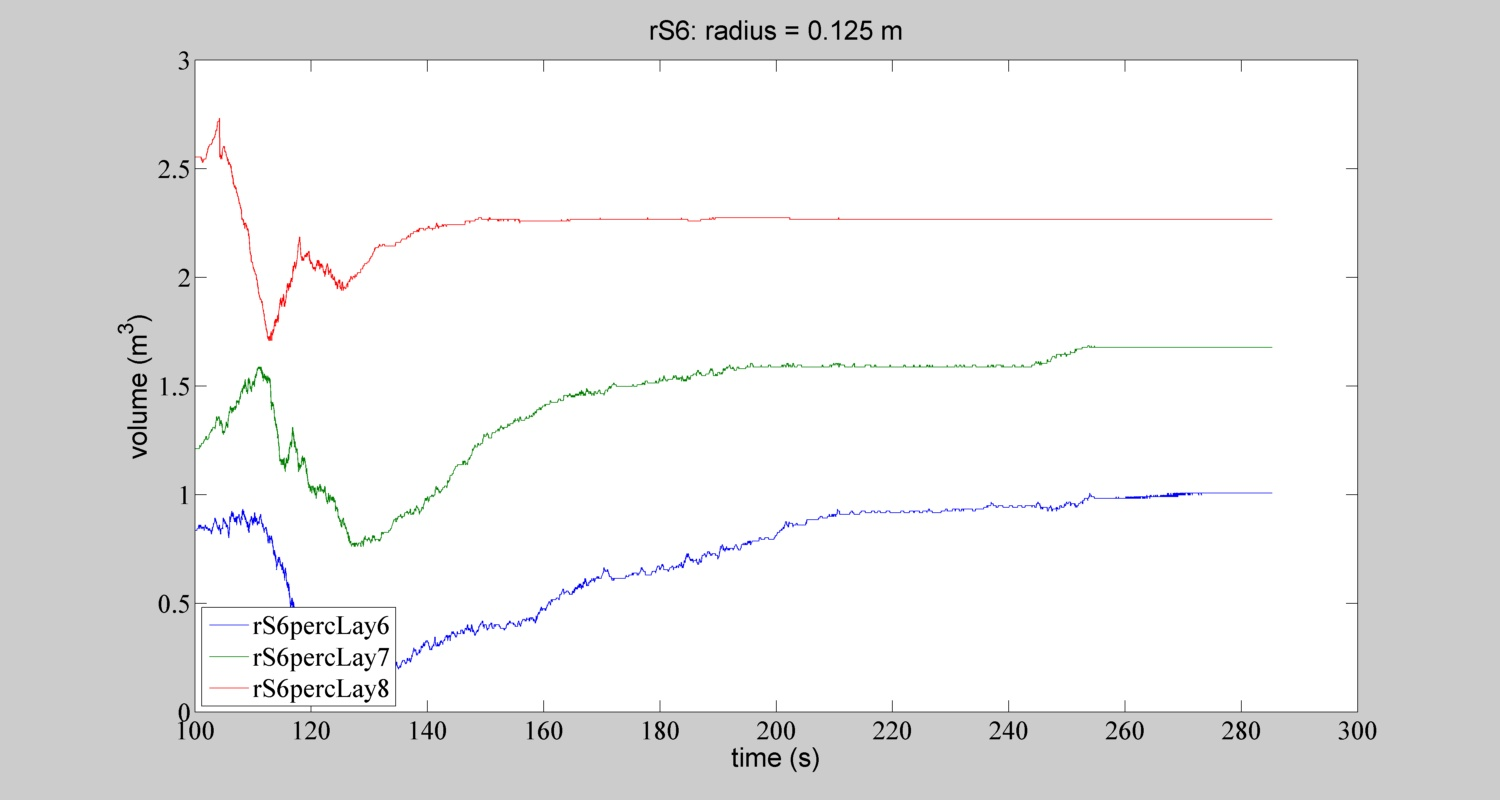
\includegraphics[width=.48\columnwidth]{images/046rS6} 
\caption{Radius 6}
\label{fig:046rS6} 
\end{figure}


\begin{figure}[!htb]
\centering
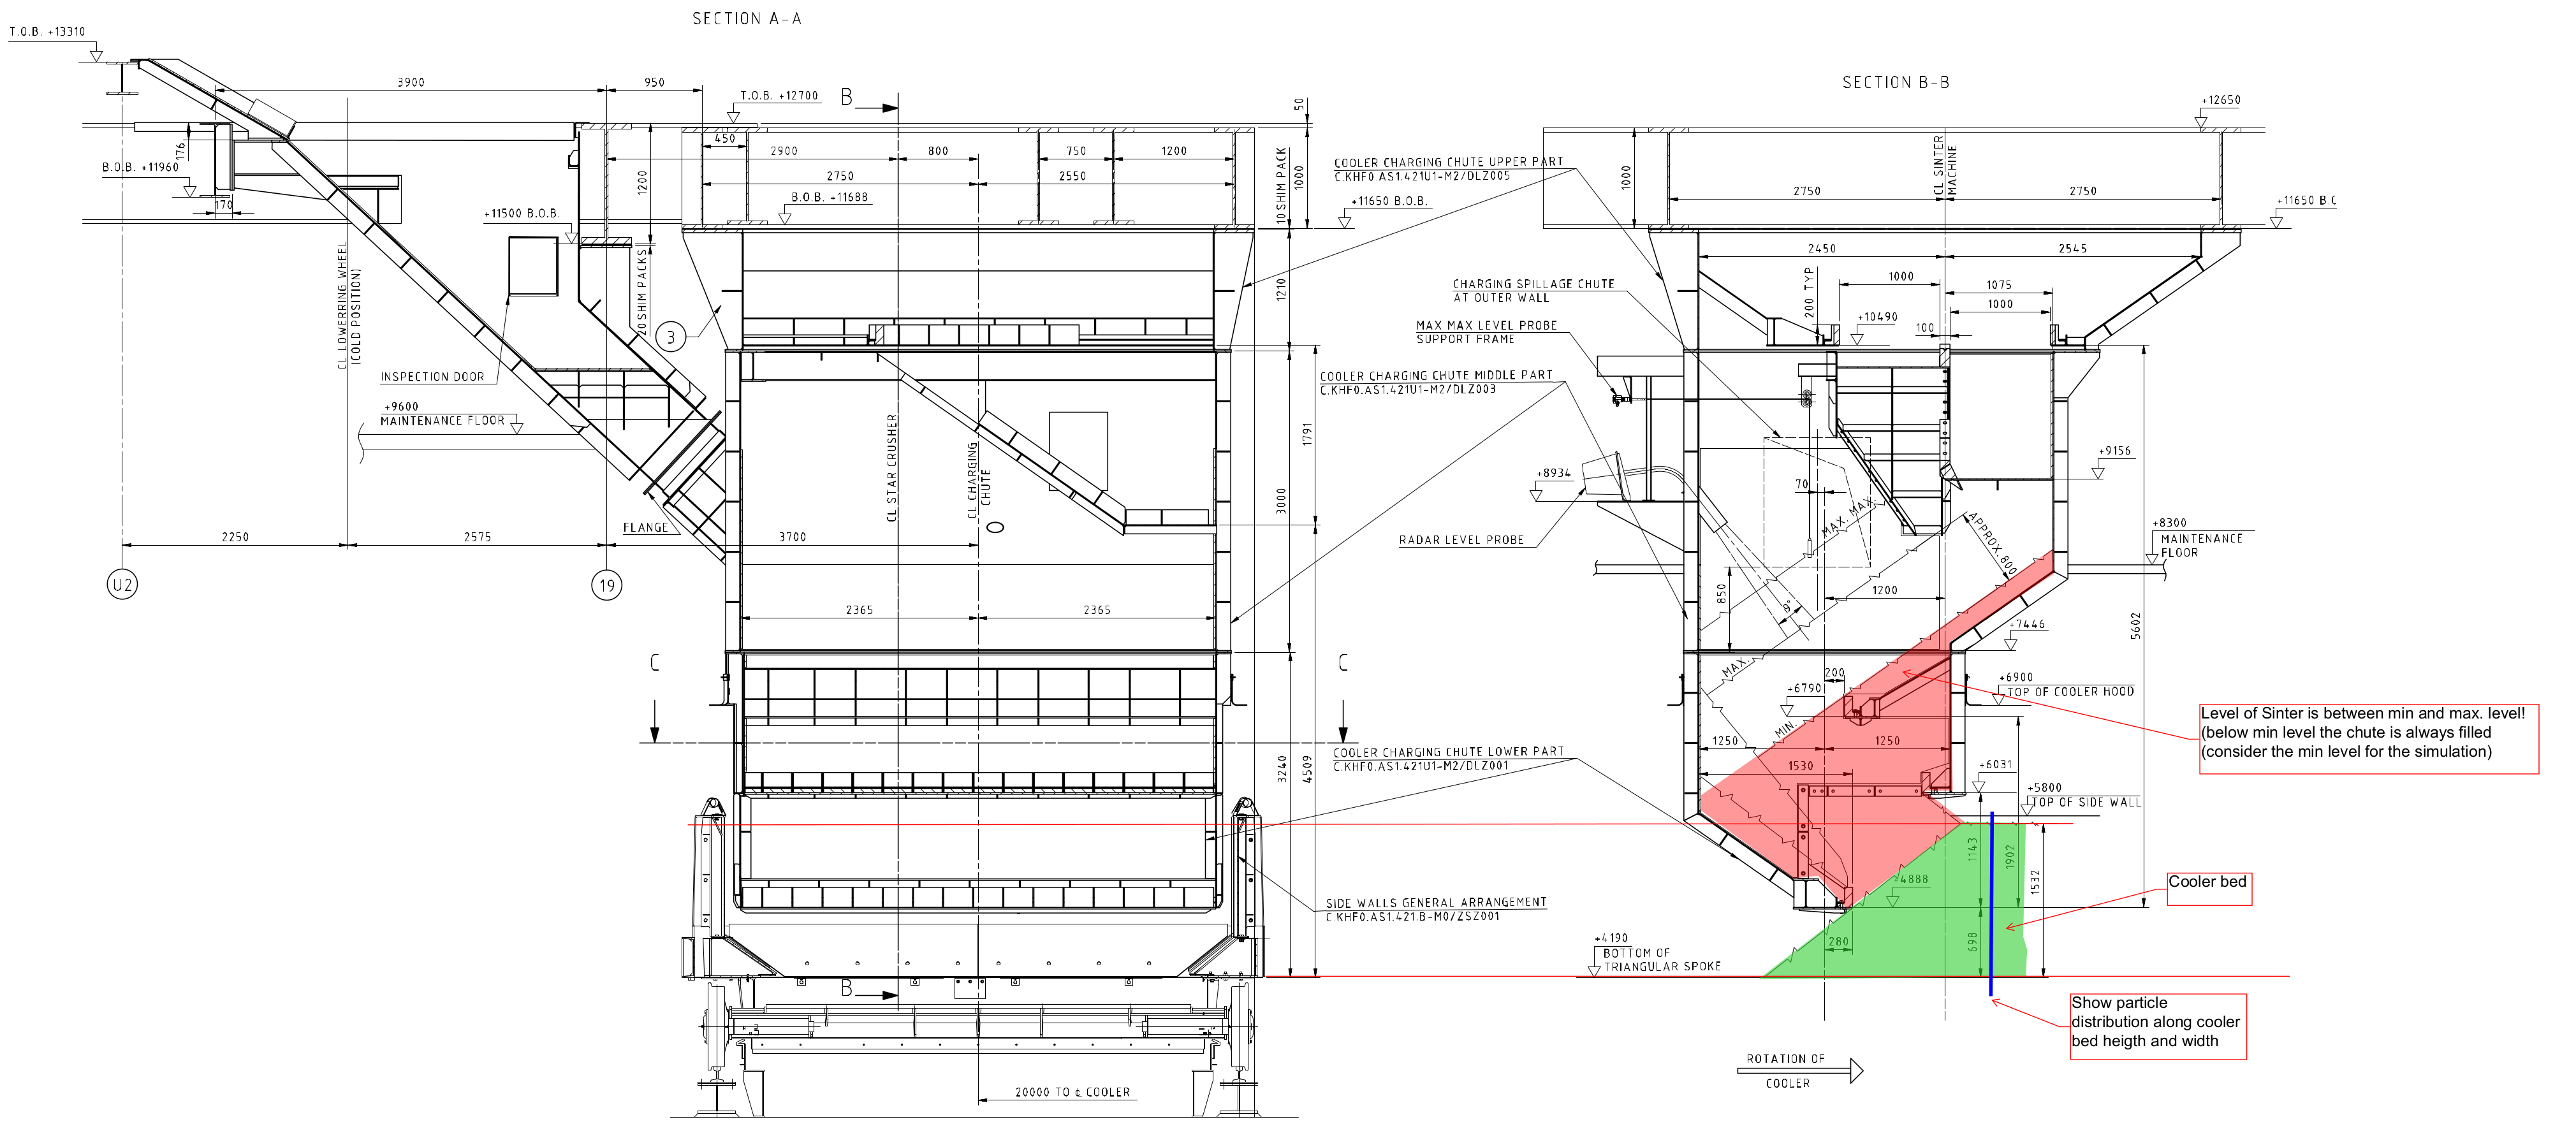
\includegraphics[width=.80\columnwidth]{055sinterChuteVerticalLayout}
\caption[Sinter chute vertical layout]{Sinter chute vertical layout.}
\label{fig:055sinterChuteVerticalLayout}
\end{figure}
\ref{fig:055sinterChuteVerticalLayout} \\

\begin{figure}[!htb]
\centering
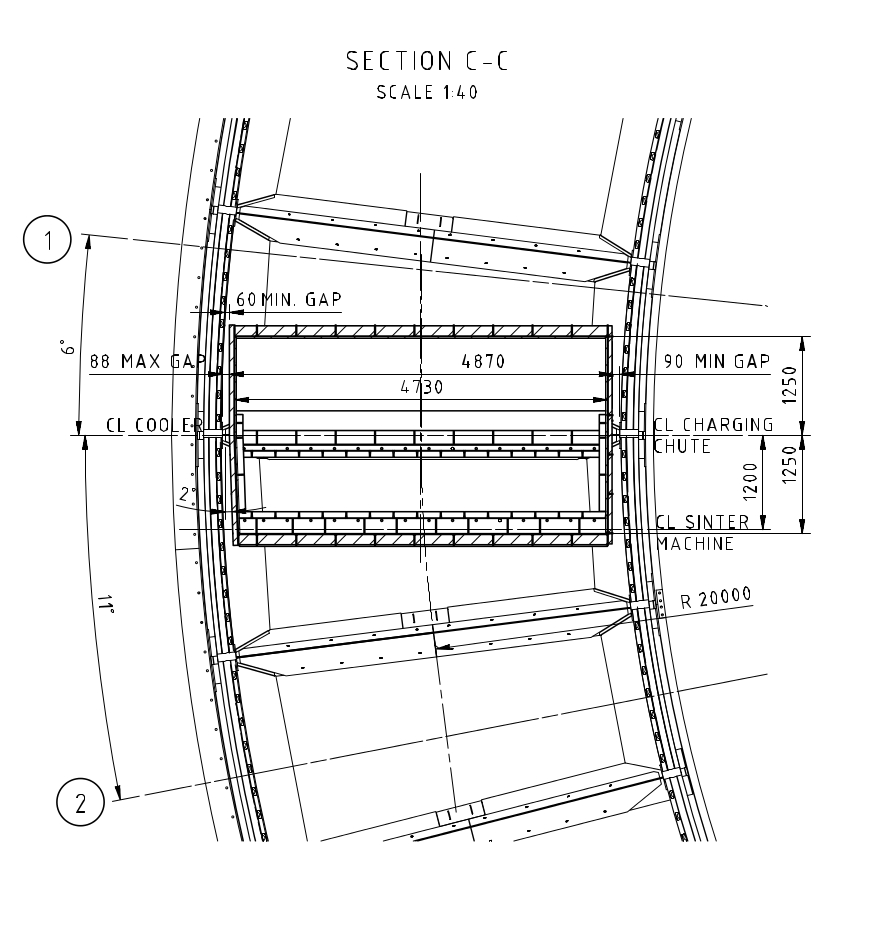
\includegraphics[width=.80\columnwidth]{images/056sinterChuteBox}
\caption[Sinter chute box]{Sinter chute box (Primetals GmbH).}
\label{fig:056sinterChuteBox}
\end{figure}
\ref{fig:056sinterChuteBox} \\


\begin{figure}[!htb]
\centering
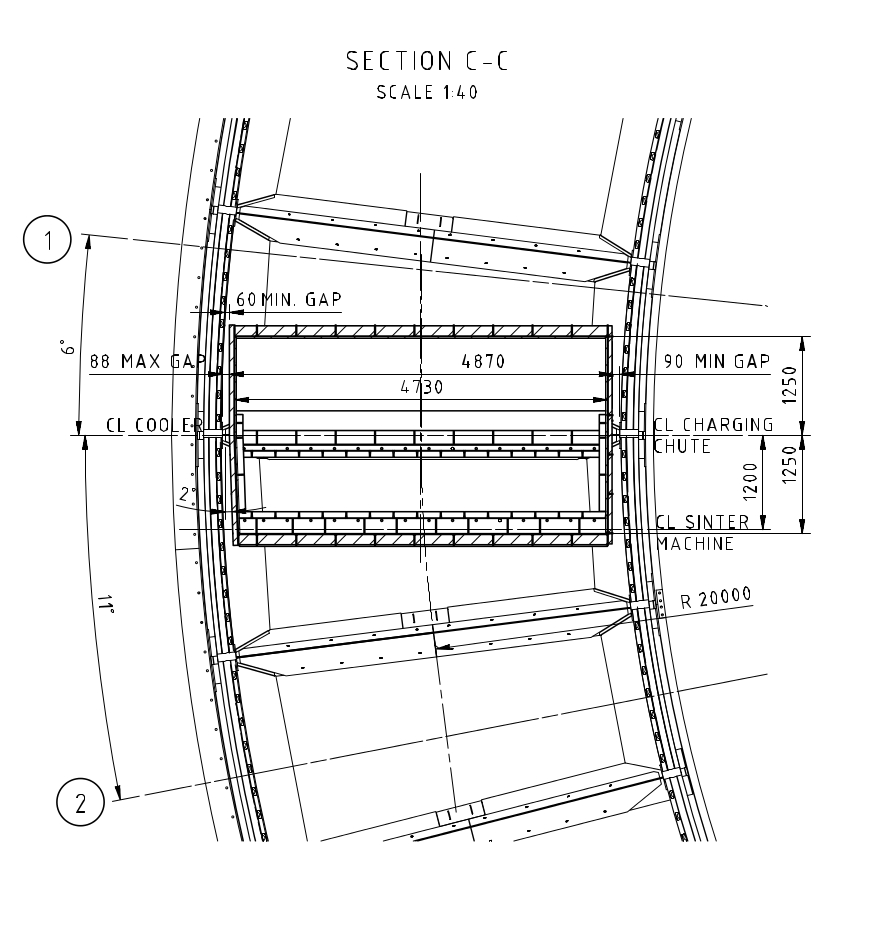
\includegraphics[width=.80\columnwidth]{images/056sinterChuteBox}
\caption[Sinter chute box]{Sinter chute box (Primetals GmbH).}
\label{fig:056sinterChuteBox}
\end{figure}
\ref{fig:056sinterChuteBox}